\section{VO2}
\subsection*{Material ID: mp-bcgk}
\textbf{Constante Dieléctrica ($\epsilon_{total}$):} 128.39 \\[0.5em]
\begin{table}[h!]
\centering
\begin{tabular}{lcc}
\toprule
\textbf{Métrica} & \textbf{Lámina (Plate)} & \textbf{Cilindros (Rod)} \\
\midrule
Bandgaps ($a/\lambda$) & [0.700 - 0.731], [0.733 - 0.744], [0.746 - 0.752], [0.754 - 0.756] & [0.822 - 0.840] \\
Resonancias & 36 & 36 \\
\bottomrule
\end{tabular}
\end{table}
\begin{figure}[H]
\centering
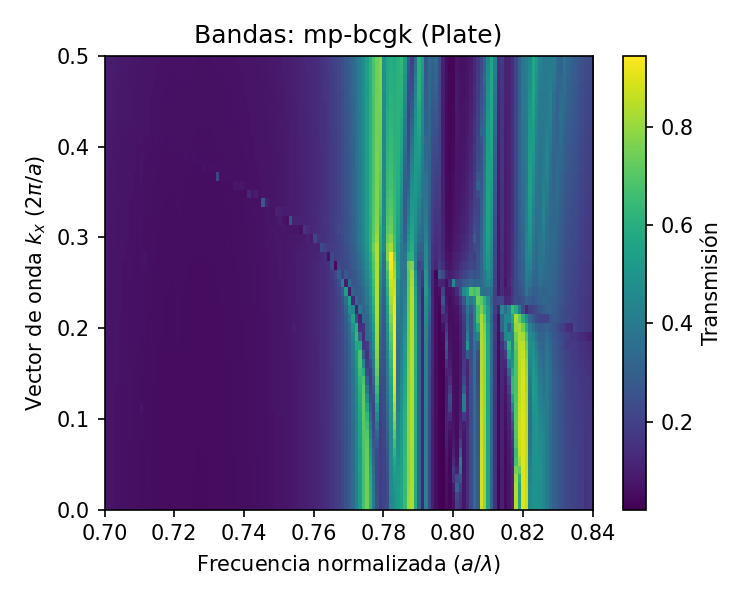
\includegraphics[width=0.48\textwidth]{figures/mp-bcgk_plate.png}
\hfill
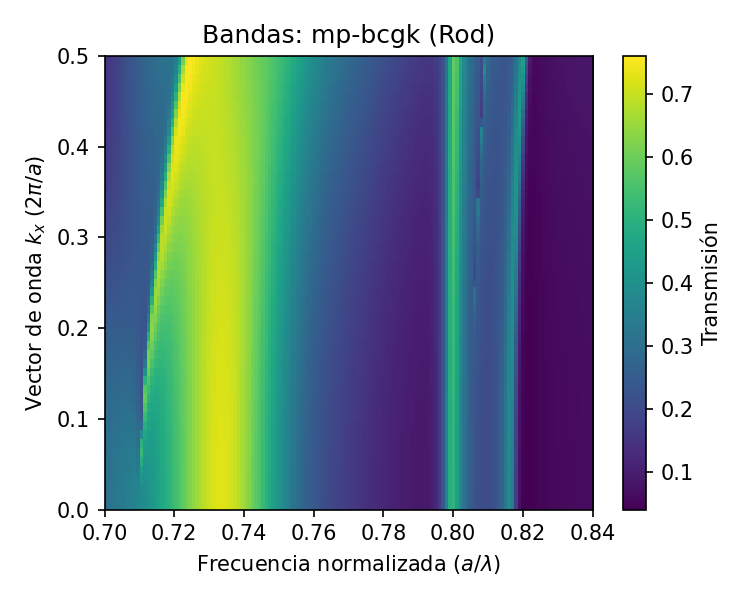
\includegraphics[width=0.48\textwidth]{figures/mp-bcgk_rod.png}
\caption{Estructuras de bandas fotónicas para mp-bcgk. Izquierda: Lámina. Derecha: Cilindros.}
\end{figure}
\vspace{1em}
\hrule
\vspace{1em}
\clearpage